\chapter{Aplikacja demonstracyjna}
\label{c6:c6}

\section{Opis aplikacji wspomagającej zarządzanie magazynem}
	\subsection{Założenia, wymagania oraz ich realizacja}
		Aplikacja przygotowana jako część praktyczna pracy dyplomowej miała za zadanie
		zobrazować niektóre z funkcji, które powinien spełniać system wspomagający
		zarządzanie gospodarką magazynową. Podstawowym wymaganiem stało się więc
		dostarczenie aplikacji dostępnej z każdego miejsca, posiadającej dostęp
		do centralnej bazy danych oraz wspartej oprogramowaniem umożliwiającym
		zaprogramowanie podstawowych algorytmów. Aplikacja jest dostępna przez interfejs przeglądarki
		internetowej, co daje możliwość korzystania na dowolnej maszynie, bez konieczności
		instalacji skomplikowanego oprogramowania. 
	\subsection{Dostępna funkcjonalność aplikacji}
		Istniejąca funkcjonalność zapewnia:
		\begin{itemize}
			\item Dostęp do funkcji aplikacji jedynie dla osób upoważnionych
			\begin{itemize}
				\item aplikacja rozpoznaje czy użytkownik jest już zalogowany
				\item użytkownik może w każdej chwili zakończyć pracę
				\item użytkownik jest automatycznie wylogowywane po 30 minutach 
			\end{itemize}
			\item Rejestracja nowego przedsiębiorstwa oraz pojedynczego magazynu;
			\item Rejestracje dowolnej ilości stref wydzielonych w magazynie, a także organizowania
			stref w strukturę drzew. Takie rozwiązanie jest elastycznym podejściem, które
			pozwala na przenoszenie ładunków między różnymi strefami, jeśli istnieje taka możliwość, tj.
			gdy strefa C jest, nie koniecznie bezpośrednim, potomkiem strefy A.
			\item Rejestracja nowych klientów: \textbf{dostawców oraz odbiorców}, którzy traktowani są
			zgodnie ze swoją funkcją w misji przedsiębiorstwa, czyli dostawca odpowiedzialny jest
			jedynie za dostawy. Niewykluczona jest sytuacja, gdy ten sam klient, jest zarówno dostawcą, jak
			i odbiorcą. 
		\end{itemize}
	\subsection{Realizacja postulatów aplikacji WMS}
		Aplikacja realizuje postulaty funkcjonalności WMS w obszarach wspomagania gospodarki magazynowej,
		ewidencji towarów, podziału magazyny na logiczne jednostki oraz utrzymania informacji
		o wydaniach / przyjęciach produktów. Odpowiednio wydanie towaru implikuje zmniejszenie stanów
		magazynowych, a przyjęcie zmniejszenie oraz alokację w strefach odkładczych.
	\subsection{Aplikacja widziana oczami programisty}
		Aplikacja wspomagająca zarządzanie magazynem została zaprojektowana i zbudowana jako aplikacja
		dostępna przez przeglądarkę. W założeniu istniało przygotowanie programu, którego będzie można
		używać na dowolnej z przeglądarek, obecnie istniejących na rynku, dzięki zastosowaniu
		narzędzi zapewniających taką kompatybilność. Cały program korzysta z architektury
		\textbf{klient - serwer - baza danych}, z silnikiem naciskiem położonym na funkcjonalność
		serwera. Część kliencka została zaprojektowana na wzór aplikacji desktop\footnote{
			\textbf{Aplikacja desktop} - aplikacja, którą można uruchomić na komputerach klasy PC,
			nie wymaga przeglądarki jako środowiska pracy, tylko odpowiednio przygotowane
			środowiska uruchomieniowego na docelowej platformie		
		} oraz zaimplementowana, w całości, przy użyciu kompletnego i zwartego framework'a\footnote{
			\textbf{Framework} - jest to całościowy zestaw bibliotek, narzędzi, a także zasad i wytycznych
			ułatwiających w znacznym sposób przygotowanie gotowej aplikacji		
		} JavaScript'owego \footnote{
			\textbf{JavaScript} - język wspierający idee programowania obiektowego i prototypowego, mający
			szerokie zastosowanie jako narzędzie wspierające wprowadzanie dynamiki do stron
			internetowych. 		
		}.
	\subsection{Architektura klient - serwer - baza danych oraz Model - Widok - Kontroler}
		\paragraph{Baza danych} jest warstwą danych dla projektu. Oparta o wolny i otwarty \footnote{
			Dostępny na licencji \href{http://www.gnu.org/licenses/old-licenses/gpl-2.0.html}{GPLv2}
		}
		serwer \textbf{MySQL}. Było to rozwiązanie podyktowane szerokim użyciem tego silnika w 
		na wielu serwisach, które umożliwiają hosting strong, czyniąc warstwę modelu danych możliwą
		do ponownego wykorzystania, bez konieczności, często problematycznego, migrowania danych do
		nowego silnika. \\
		Warto w tym miejscu wspomnieć o kolejnym narzędziu, które mimo, że działa na poziomie serwera, 
		odpowiada za dostarczenie odpowiedniej abstrakcji dla warstwy modelu danych i ułatwienia
		operacji nań. Wspomnianym narzędziem jest ogólnodostępne i otwarto źródłowy projekt Hibernate. 
		Konfiguracja jest oparta na co najmniej jednym pliku, tak jak na załączniku \ref{appendix:hibernateCfg}. 
		\paragraph{Serwer} został napisany w całości w języku Java i oparty o kontener aplikacji webowych 
		\textbf{Tomcat}\footnote{
			\textbf{Apache Tomcat} - serwer aplikacji internetowych, którego główną częścią jest interakacja
			ze specjalnymi klasami znanymi jako \textit{servlety}, umożliwiających korzystanie z funkcjonalności
			jaką oferuje serwer przez standardowy protokół \textit{HTTP} i żądania \textit{CRUD}		
		}, a sama podstawową zasadą przy jego tworzeniu było oparcie centralny punkt wejściowy - fasadę, która dawała
		dostęp do całej funkcjonalności aplikacji przez zwarty interfejs, decydujący o wyborze konkretnego rozwiązania.
		
		Parametr typu \textbf{CRUD} przyjmuje jedną z 4 wartości:
		\textit{Create, Read, Update, Delete} zależnie od metody żądania HTTP, która go wywoła. Jest to najprostsza rzecz
		do ustalenia, ale prawdopodobnie jedna z najważniejszych. Znając jej wartość algorytm jest w stanie wywołać
		odpowiednie metody odpowiedzialne za obsługę zgłoszenia. Przykładowo, sytuacją oczekiwaną na żądania 
		\textit{GET} byłoby wystosowanie zgłoszenia do warstwy modelu danych, aby ta zwróciła zbiór wartości odpowiadających
		warunkom, jakie serwer odebrał od aplikacji klienckiej. 
		
		\begin{table}
			\begin{tabular}[c]{l*{2}{c}}
				Żądanie HTTP	& 	wartość zmiennej typu CRUD	\\
				\hline
				POST			&	CREATE						\\
				PUT				& 	UPDATE						\\
				DELETE			&	DELETE						\\
				GET				& 	READ						\\
			\end{tabular}
			\label{c6:tab:CRUD_matches}
			\caption[Żądania HTTP a enum CRUD]{Odpowiednie wartości enuma \textit{CRUD}, a żądania HTTP}
		\end{table}
		\begin{listing}[h]
			\inputminted[
				linenos=true,
				fontsize=\tiny,
				firstline=57, 
				lastline=75,
	            numbersep=15pt
			]{java}{../application/javaSrc/wms/servlet/WMSDataAgent.java}	
			\label{c6:listing:WMSDataAgent}
			\caption[WMSDataAgent - \textbf{processRequest}]{\textit{WMSDataAgent-processRequest} - 
			metoda rozdzielająca zadania na podstawie adresu oraz metody CRUD}
		\end{listing}
		\begin{listing}[h]
			\inputminted[
				linenos=true,
				fontsize=\tiny,
				firstline=32, 
				lastline=45,
	            numbersep=15pt
			]{java}{../application/javaSrc/wms/controller/base/extractor/RDExtractor.java}	
			\label{c6:listing:WMSDataAgent}
			\caption[RDExtractor - \textbf{parse}]{\textit{RDExtractor-parse} - metoda parsująca żądania HTTP i zwracające 
			potrzebne opcje jako obiekt}
		\end{listing}		
		
		\paragraph{Klient}
\section{Diagramy, zrzuty ekranowe oraz funkcje}
	\subsection{Logowanie do aplikacji przy pierwszym uruchomieniu}
		\begin{figure}[H]
			\centering
			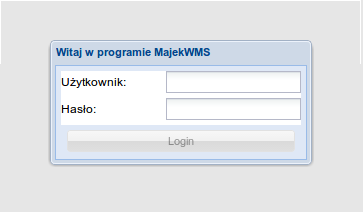
\includegraphics[width=0.99\textwidth]{images/app/login}
			\caption[Aplikacja - Logowanie do programu]{Zrzut ekranu pokazują aplikację w stanie tuż po uruchomieniu}
			\label{c7:fig:app:login}
		\end{figure}
		
	\subsection{Zarządzanie strukturą magazynu}
		\begin{figure}[H]
			\centering
			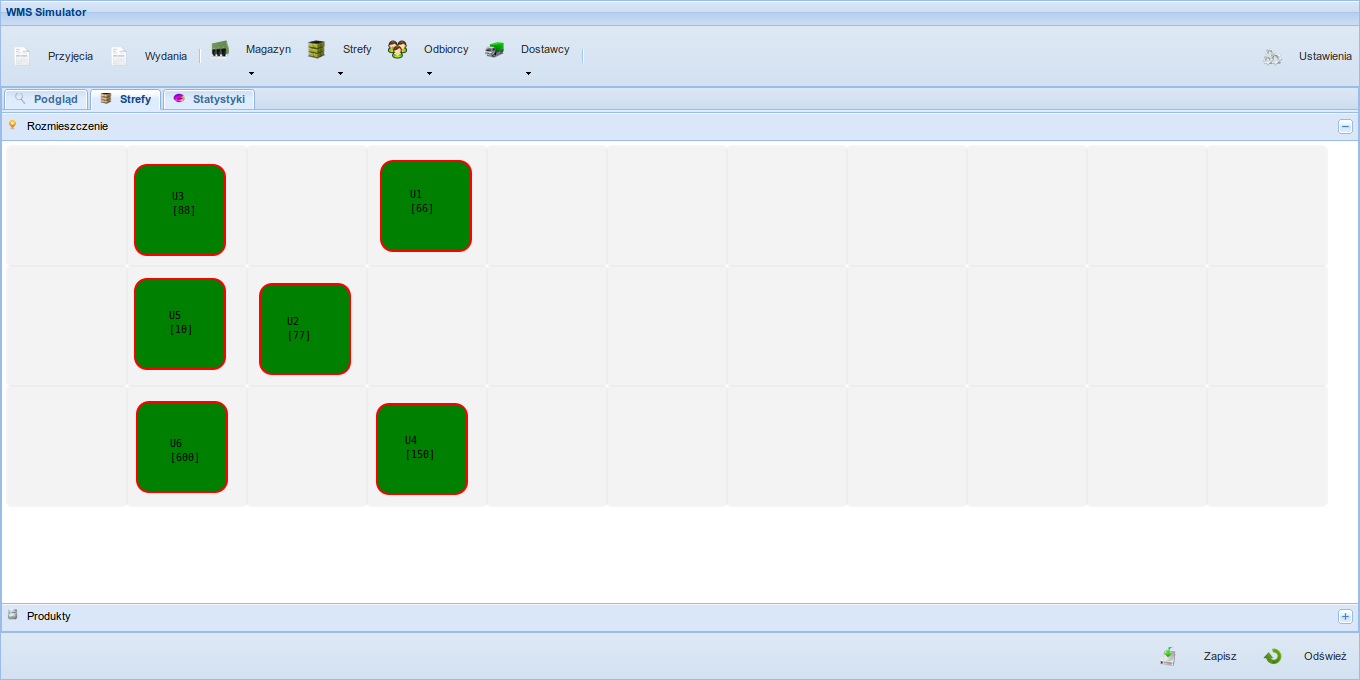
\includegraphics[width=0.99\textwidth]{images/app/unit_preview}
			\caption[Aplikacja - Zarządzania strukturą magazynu]{Zrzut ekranu z widokiem na strukturę magazynu}
			\label{c7:fig:app:unit_preview}
		\end{figure}
		
	\subsection{Zarządzanie klientami - dodawanie, usuwaniu, edycja oraz podgląd}
		\begin{figure}[H]
			\centering
			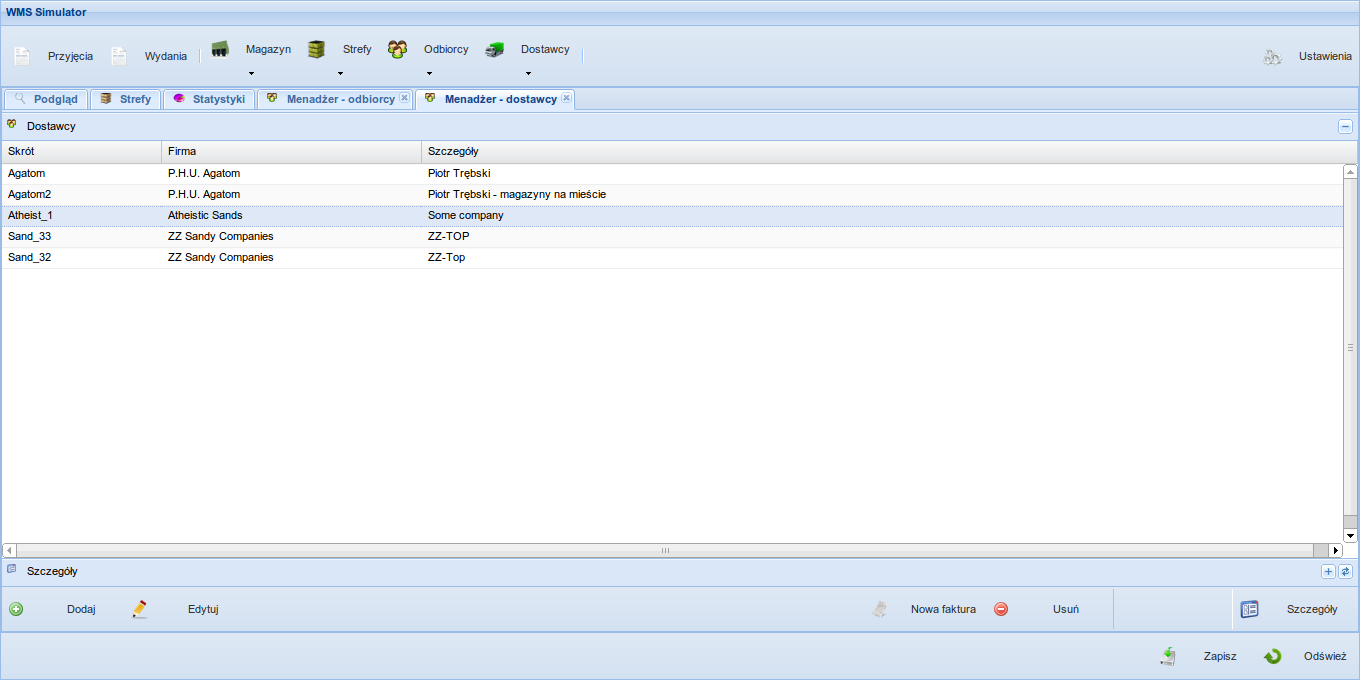
\includegraphics[width=0.99\textwidth]{images/app/supplier_preview}
			\caption[Aplikacja - Dostęp do danych klientów]{Zrzut ekranu z widokiem na dostępnych dostawców}
			\label{c7:fig:app:supplier_preview}
		\end{figure}
		\begin{figure}[H]
			\centering
			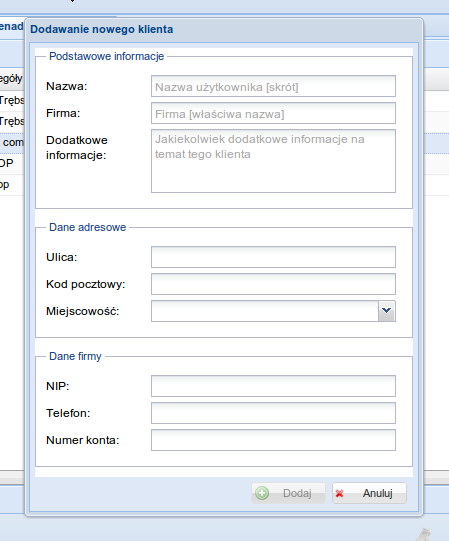
\includegraphics[width=0.6\textwidth]{images/app/new_receipient_dialog}
			\caption[Aplikacja - Dodawania nowego klienta - odbiorcy]{Zrzut ekranu z widokiem na okno dialogowe dla tworzenia nowego odbiorcy}
			\label{c7:fig:app:new_receipient_dialog}
		\end{figure}
		
	\subsection{Wydanie, przyjęcia oraz ewidencja produktów}
		\begin{figure}[H]
			\centering
			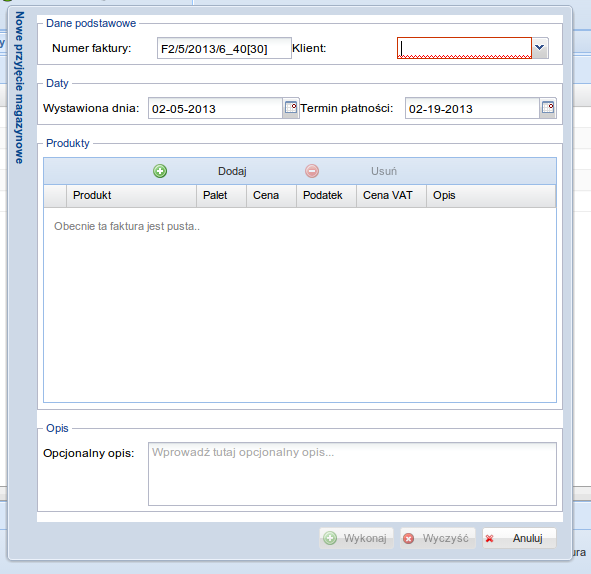
\includegraphics[width=0.99\textwidth]{images/app/new_supply_preview}
			\caption[Aplikacja - Dodanie nowego dokumentu wydania]{Zrzut ekranu z widokiem na kreator nowego wydania magazynowego}
			\label{c7:fig:app:new_supply_preview}
		\end{figure}
		\begin{figure}[H]
			\centering
			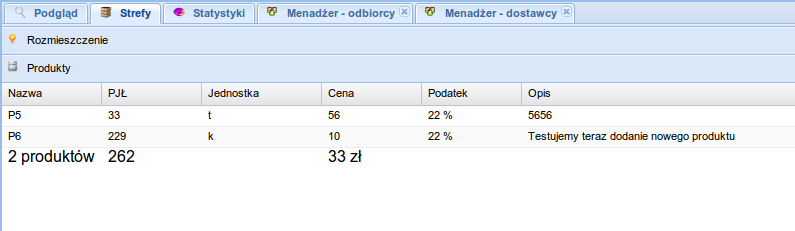
\includegraphics[width=0.8\textwidth]{images/app/unit_products_preview}
			\caption[Aplikacja - Ewidencja towarów w poszczególnych strefach]{Zrzut ekranu z widokiem listy produktów w wybranej strefie}
			\label{c7:fig:app:unit_products_preview}
		\end{figure}